\documentclass[12pt]{article}

\usepackage{graphicx}
\usepackage{url}

\usepackage{fancyhdr}
\usepackage[T1]{fontenc}
\usepackage[polish]{babel}
\usepackage[utf8]{inputenc}
\usepackage{lmodern}
\usepackage{caption}
\selectlanguage{polish}
\usepackage{listings}
\title{My first document}
\date{2013-09-01}
\author{Kamil Warpechowski}


\fancypagestyle{firststyle}
{
   \fancyhf{}
   \fancyfoot[C]{
		Warszawa, \today
   }
}

\begin{document}


\thispagestyle{firststyle}
\begin{center}

\includegraphics[width=1\textwidth]{images/logo.jpg}
\textbf{Wydzial Informatyki} \\
\vspace{3em}
\textbf{Katedra Sieci Komputerowych} \\
Sieci Urządzeń Moblinych \\
\vspace{3em}
\textbf{Kamil Warpechowski} \\
Nr albumu 10709
\end{center}


\vspace{3em}
{\addtolength{\leftskip}{70mm}

\noindent
Praca inżynierska
\\Promotor:
\\dr inż. Michał Tomaszewski

}

\vspace{3em}

\textbf {
	tutaj będzie zajebisty tytuł
}



  \newpage
  
  
  \tableofcontents
  \newpage
  

\section{Wprowadzenie}

Hello World!


\section{Cel pracy}
xx
\section{Rozszerzona rzeczywistość}

\begin{center}
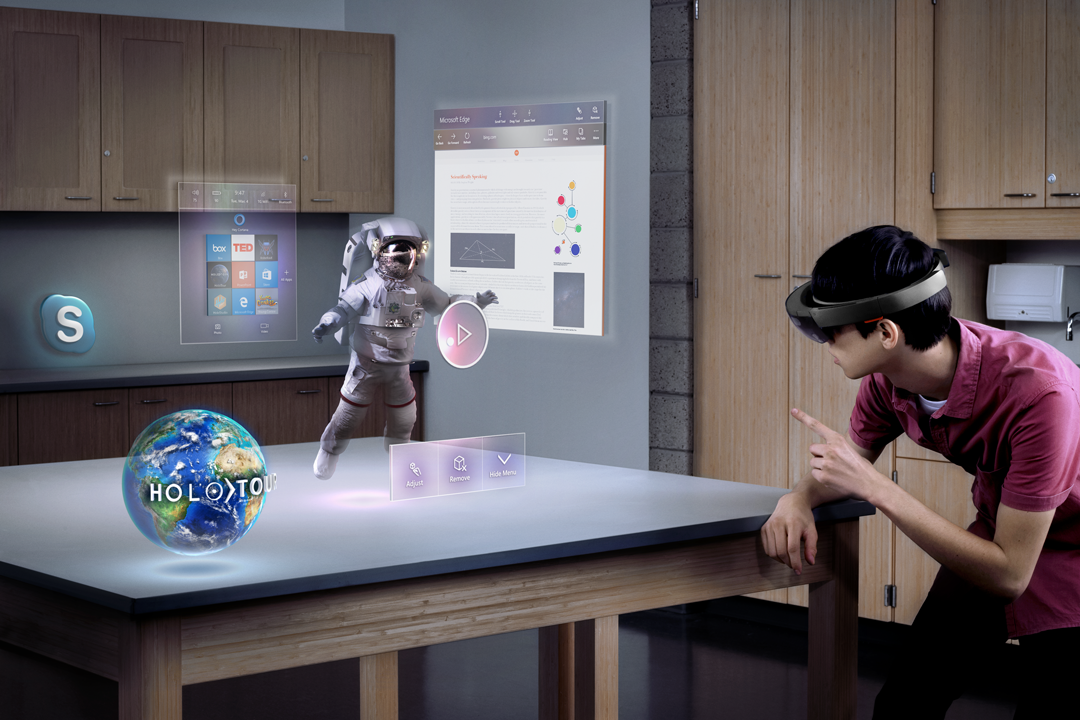
\includegraphics[width=0.8\textwidth]{images/hololens.png}
\captionof{figure}{
Wizualizacja Microsoft HoloLens
}
\small {źródło: https://www.microsoft.com/microsoft-hololens/en-us/why-hololens }
\end{center}

\section{Wykorzystane technologie}

\subsection{Unity}
Unity jest obecnie najpopularniejszą platformą do tworzenia gier na wiele platform. 
\subsubsection{Dlaczego Unity}
Najnowsza wersja posiada natywne wsparcie do rozszerzonej oraz wirtualnej rzeczywistości. Narzędzie te posiada prosty, ergonomiczny interfejs co ułatwia pracę.\\
Logikę biznesową oraz skrypty pomocnicze można pisać w języku C\#. Jest to duże udogodnienie, gdyż jest ów język posiada wiele wbudowanych klas (np. do obsługi połączęń TCP) oraz niezliczoną ilość bibliotek.
Bardzo pomocnym dodatkiem do narzędzia jest ,,Assets Store''. Jest to wirtualny sklep z komonentami do tworzenia gry. W projekcie zastosowałem tekstury i obiekty 3d pochodzące z tego źródła.
\subsubsection{Alternatywne rozwiązania}


 \begin{tabular}{|c|c|c|}
 \hline
 \ & Unity & Unreal Engine \\ 
  \hline
 Wsparcie języków programowania & C Sharp, JavaScript, Boo & c++ \\  
  \hline
 Obsługa wielu ekranów & Tak & Nie \\
 \hline  
  &  &  \\
  \hline   
  &  &  \\
  \hline   
  &  &  \\
  \hline   
\end{tabular}
\captionof{table}{Porównanie silników gier}

\subsection{Android}

\subsection{Połączenie sieciowe}

\subsubsection{Alternatywne rozwiązania}


\section{Aplikacja główna}
\subsection{Logika biznesowa}
\subsection{Serwer komunikacyjny}
\section{Aplikacja mobilna - kontroler}


\begin{lstlisting}[language=Java]
String s = new String();
\end{lstlisting}

 
\newpage
\thispagestyle{empty}
 
  
\listoffigures
 
\listoftables
\begin{thebibliography}{99}
\bibitem{pa} H.~Partl:
\emph{German \TeX},
TUGboat Vol.~9,, No.~1 ('88)
\end{thebibliography}

\end{document}